\documentclass{article}
\usepackage[T1]{fontenc}
\usepackage[portuguese]{babel}
%\usepackage[htt]{hyphenat}
\usepackage{amsmath}
\usepackage{times}
\usepackage{color}
\usepackage{anppom2008}

\newcounter{notecounter}

\newcommand{\note}[1]{
  \addtocounter{notecounter}{1}
  \textcolor{red}{[note \arabic{notecounter}: #1]}
}

\newcommand{\rameau}{\textit{Rameau}}

\begin{document}
\graphicspath{{figs/}}

\title{Título do trabalho}
\author{Autor}{Filiação acadêmica}{e-mail}{website}

\begin{sumario}
  Resumo do texto com até 100 palavras.  
\end{sumario}

\keywords{até cinco palavras-chave que descrevam o assunto do texto}

\section{Introdução}
\label{sec:introducao}


\section{Rameau}
\label{sec:rameau}

Todo o trabalho descrito nesse artigo foi desenvolvido usando o
sistema \rameau{} \footnote{Èstá descrito em outro trabalho do autor,
  a citação foi removida por anonimato e será acrescentada na ocasião
  da publicação.} para análise automática de harmonia e extração de
informação musical. \rameau{} é um framework para implementação de
algoritmos de análise harmônica de partituras simbólicas. As
partituras são guardadas em arquivos no formato Lilypond
\cite{nienhuys.ea08:lilypond}, que permite diferenciação de notas
enarmônicas e geração de partituras bem tipografadas. As notas são
extraídas das partituras e apresentadas a uma rede neural, que associa
cada conjunto de notas a um acorde. Para esse trabalho, o \rameau{}
foi extendido para realizar operações comuns de musicologia, como
detecção de cruzamentos, quintas ou oitavas consecutivas, cadências
frequentes, etc.

Além disso \rameau{}  possui vários outros algoritmos para análise
harmônica, como o de Pardo e Birmingham \cite{pardo.ea00:automated},
outras redes neurais e classificadores de árvores de decisão e
k-vizinhos-mais-próximos. Atualmente \rameau{}  está sendo extendido para
realizar análise funcional de qualquer peça tonal.

Os corais utiliados nesse artigo foram extraídos do formato MIDI para
o lilypond por uma ferramenta automática e depois corrigidos
manualmente para remover erros de enarmonia e notas incorretas. Usamos
gabaritos manuais de análise harmônica para validar os algoritmos de
análise, e o algoritmo escolhido para análise de cadências encontra
corretamente em torno de 98\% dos acordes\footnote{Idem.}.

\section{Metodologia}
\label{sec:metodologia}

366 dos 371 corais

KP e no singular (no sentido de ``o livro sugere'')

\section{Análise}
\label{sec:analise}

\subsection{Âmbitos}
\label{sec:ambitos}

Os corais de Bach foram escritos para serem cantados por músicos
profissionais e não pela congregação \cite{bach41:371}. Isso \note{nao
  começa com isso} se reflete na textura, cruzamentos e no âmbito
vocal usado nos corais. A figura \ref{fig:ambito-kostka} mostra os
âmbitos sugeridos por KP e os utilizados por Bach nos corais
analizados. Bach amplia o âmbito de soprano e teror em uma segunda
maior ascendente, e o do contralto em uma segunda maior descendente. A
voz do baixo tem ampliação de uma terça maior em ambas direções
(comparando com KP). A tabela \ref{tab:notas-extremas} lista os corais
onde as notas mais agudas e graves ocorrem em cada voz.

\begin{table}[t]
\begin{center}
\begin{small}
\begin{sc}
  \begin{tabular}{r|p{4cm}p{4cm}}
    & nota mais aguda & nota mais grave \\ 
    \hline
    soprano &  116 254 282 298 331 334 &  186 034 050 068 075 223 049 070 100 165 185 197 214 325 348 158 175
    205 239 352 087 110 244 \\ \aroundspace
    contralto & 024 028 033 036 057 058 069 078 084 123 217 225 248 252 329 331 334
    354 359 &   345 186 \\ \aroundspace
    tenor &   024 043 074 083 151 156 224 248 263 264 273 276 281 329
    354 371 &   229 070 205 \\ \aroundspace
    baixo &   285 312 331 &   034 051 214 223 340 131 328 143 155 197 205 219 241 187 235 319 337
    240 070 075 165 175 239 
  \end{tabular}
  \caption{Corais com notas extremas}
  \label{tab:notas-extremas}
\end{sc}
\end{small}
\end{center}
\end{table}

\begin{figure}
  \centering
  \includegraphics[scale=2.5]{ambitos}
  \caption{Comparação de âmbito utilizado por Bach e definido por Kostka e Payne}
  \label{fig:ambito-kostka}
\end{figure}

\subsection{Cruzamento de vozes}
\label{sec:cruzamento-de-vozes}

Dos corais analizados 209 tem cruzamentos entre as vozes (57\%). KP
sugere evitar cruzamentos, principalmente acima do soprano ou abaixo
do baixo. Eles permitem o cruzamento breve das linhas de contralto e
tenor se existir uma razão musical \cite[p. 79]{kostka.ea00:tonal}. De
fato, dos corais com cruzamento, o cruzamento mais comum é entre tenor
e contralto (64,6\%), mas o cruzamento entre tenor e baixo é quase tão
comum (60\%). O cruzamento entre contralto e soprano é menos frequente
(14,8\%) mas existente, contrariando a regra de não cruzar acima do
soprano. De qualquer forma, a grade maioria (85\%) dos cruzamentos são
curtos (nunca maiores que dois tempos). A análise de cruzamentos
mostra alguns exemplos interessantes: no coral 35 o contralto é a voz
mais grave por um breve periodo de tempo (as vozes do tenor e baixo estão
acima da voz do contralto) \note{fig}, e no coral 290 existe um
cruzamento simultâneo de baixo com o tenor e do contralto com o
soprano \note{fig}.

% \begin{figure}
%   \centering
%   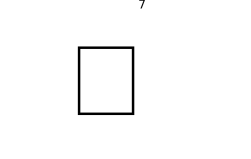
\includegraphics{coral-003}
%   \caption{aa}
%   \label{fig:coral-003}
% \end{figure}

Os cruzamentos podem ser classificados em duas categorias; para evitar
quintas e oitavas consecutivas \note{fig} e para manter melhor
condução de vozes \note{fig}. Contudo inúmeros cruzamentos poderiam
ser evitados. 

Em alguns corais com cruzamento entre baixo e tenor, por exemplo 29,
35 e 76, a edição usada sugere atravém de uma \textit{ossia} que as
notas do baixo sejam cantadas uma oitava abaixo para evitar o
cruzamento. Essa sugestão levanta a questão do porque Bach não
escreveu as notas nessa oitava em primeiro lugar.

\subsection{Saltos melódicos}
\label{sec:saltos-melodicos}


\subsection{Quintas e oitavas consecutivas}
\label{sec:quintas-e-oitavas}

Apesar do uso de quintas e oitavas consecutivas ser relativamente
comum na escrita instrumental, seu uso constitui uma das regras mais
básicas a ser evitada no estudo de harmonia e contraponto. Dessa
maneira, é interessante verificar quantas oitavas e quintas
consecutivas existem nos corais de Bach. O número de oitavas e quintas
juntos é pouco representativo (4\%) em comparação com todos os corais
analisados. Existem 8 quintas e 7 oitavas consecutivas.

Algumas dessa quintas e oitavas ocorrem entre o último acorde de uma
frase e primeiro acorde da próxima. Isso ocorre nos corais 45 e 46
(quintas) e 2, 89, e 279 (oitavas). \note{fig} Uma possível
justificativa é a ``quebra'' de uma frase para outra. Contudo, a
maioria das quintas e oitavas consecutivas (9 no total) ocorrem no
meio de frases. Todas as oitavas nessa categoria são uníssono--oitava
ou oitava--uníssono \note{fig}. Para o alívio dos professores de
harmonia, nenhuma dessas oitavas é paralela, mas algumas das quintas
são: nos corais 4, 46, 71, 266.

\begin{figure}
  \centering
  \subfigure[Coral 244]{
    \includegraphics[scale=5]{244-oitava}
  }
  \qquad
  \subfigure[Coral 279]{
    \includegraphics[scale=2.7]{279-oitava}
  }
  \qquad
  \subfigure[Coral 329]{
    \includegraphics[scale=2.8]{329-oitava}
  }
  \caption{Oitavas e uníssonos}
  \label{fig:oitavas-e-unissonos}
\end{figure}

\subsection{Acordes de sexta aumentada}
\label{sec:acordes-de-sexta}

Os corais apresentam exatamente três acordes de sexta aumentada e
exatamente um de cada tipo listado por KP: um acorde de sexta
aumentada alemã, um acorde de sexta aumentada italiana, e um acorde de
sexta aumentada francesa \note{fig}.

\subsection{Sétimas}
\label{sec:setimas}

acorde de passagem

bizarro

arpejo

perde sétima

ascendente

(ver setimas koechlin)

\begin{figure}
  \centering
  \subfigure[Ascendente cromática]{
    \includegraphics[scale=3]{003-setima-asc-crom}
  }
  \subfigure[Vozes de passagem]{
    \includegraphics[scale=5]{015-setima-acorde-pass}
  }
  \subfigure[Arpejo antes da resolução]{
    \includegraphics[scale=3]{049-setima-arpejo}
  }
  \subfigure[Sétima transformada em nota do acorde seguinte]{
    \includegraphics[scale=5]{120-setima-koechlin}
  }
  \caption{Resoluções de sétima}
  \label{fig:setima-resol}
\end{figure}

\subsection{Cadências finais}
\label{sec:cadencias}

O programa identifica 79\% das cadências finais (isso é, os três
ultimos acordes diferentes) com o formato $x$ V I onde $x$ pode ser ii
(menor ou diminuto), IV (maior ou menor), V/V (dominante secundária),
ou I (maior ou menor) e último acorde pode ser maior ou menor.

A cadência mais comum é do tipo II V I (36\%), seguida por I V I
(32\%). As cadências IV VI (6\%) e V/V V I (5\%) são estatisticamente
insignificantes. Apenas 3\% dos corais tem a cadência vii°/V V I, e
apenas 2\% to tipo viiø V I.

Apesar do algoritmo para analisar as cadências finais ser
relativamente ingênuo, ele identifica de maneira errada 16\% dos
corais. Por exemplo, a cadência final do coral 362 é I$^6_4$ V7 I, mas
o algoritmo interpreta a antecipação para a terça do acorde final como
um acorde menor do terceiro grau (iii). Além disso, como o algoritmo
sempre considera que o acorde final é de tônica, ele classifica
eroneamente os corais que terminam em acordes diferentes da tônica,
como os que terminam em meia-cadência.

\section{Avaliação}
\label{sec:avaliacao}

\section{Conclusão e trabalhos futuros}
\label{sec:concl-e-trab}

\renewcommand{\refname}{Referências Bibliográficas}
\bibliographystyle{kchicago}
\bibliography{writing-style,harmonic-analysis,melodic-contour,music-harmony-and-theory,programs,music-scores,genos}

\end{document}
